\chapter{Pagerank}

\section{Analiza PageRank}

W ramach analizy rangi stron w grafie WWW zaimplementowano iteracyjny algorytm PageRank, działający w wersji z tłumieniem i bez tłumienia. Obliczenia przeprowadzono dla różnych wartości współczynnika tłumienia $d$ oraz porównano otrzymane rozkłady PageRanku z rozkładem potęgowym.

\subsection{Rozkład PageRank bez tłumienia ($d = 1.0$)}

W przypadku wyłączenia tłumienia, cały przepływ PageRanku opiera się na strukturze linków — węzły końcowe (bez wyjścia) powodują akumulację rankingu. Uzyskano:

\[
\text{Regresja log-log: } y \sim x^{-1.67}, \quad R^2 = 0.868
\]

\begin{figure}[H]
\centering
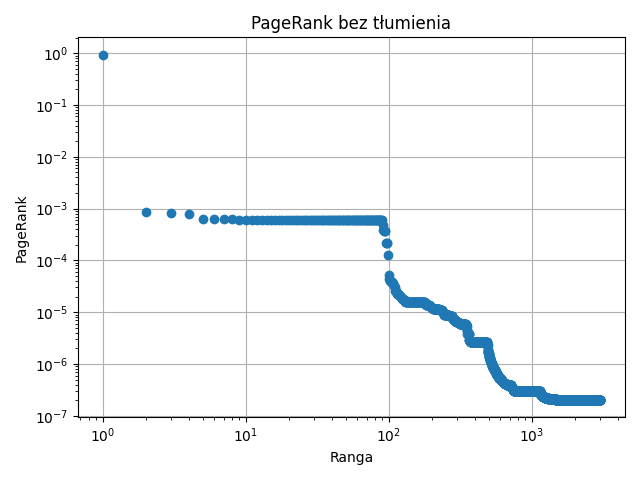
\includegraphics[width=0.6\textwidth]{assets/img_54.png}
\caption{Rozkład PageRank bez tłumienia ($d=1.0$)}
\end{figure}

\subsection{Rozkład PageRank z tłumieniem ($d = 0.85$)}

Przy zastosowaniu tłumienia (domyślna wartość $d=0.85$) uzyskano:

\[
\text{Regresja log-log: } y \sim x^{-0.83}, \quad R^2 = 0.746
\]

\begin{figure}[H]
\centering
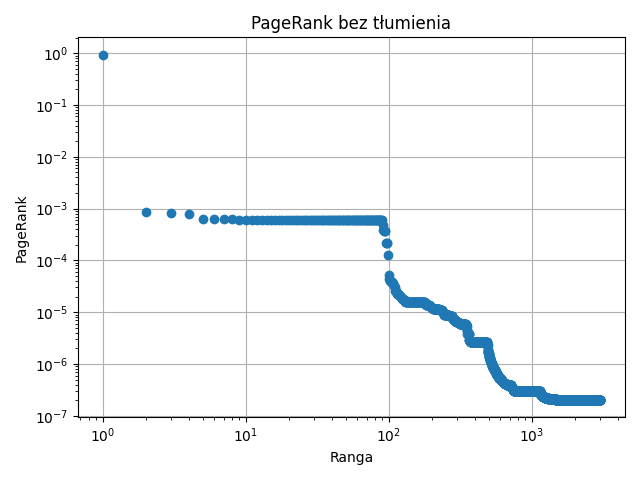
\includegraphics[width=0.6\textwidth]{assets/img_55.png}
\caption{Rozkład PageRank z tłumieniem ($d=0.85$)}
\end{figure}

Top 5 stron o najwyższym PageRank:
\begin{itemize}
    \item \url{https://www.um.edu.mt/} \quad (0.14197)
    \item \url{https://www.um.edu.mt...} \quad (0.0103)
    \item \url{http://www.um.edu.mt/privacy...} \quad (0.0100)
    \item \url{https://www.um.edu.mt/privacy/...} \quad (0.0093)
    \item \url{https://www.um.edu.mt/students/...} \quad (0.0075)
\end{itemize}

\subsection{Zbieżność PageRank dla różnych wartości tłumienia}

\textbf{Damping = 0.6}

\begin{itemize}
    \item Top 5 stron — max PR: 0.04407
    \item Regresja log-log: $x^{-0.58}$, $R^2 = 0.667$
\end{itemize}

\begin{figure}[H]
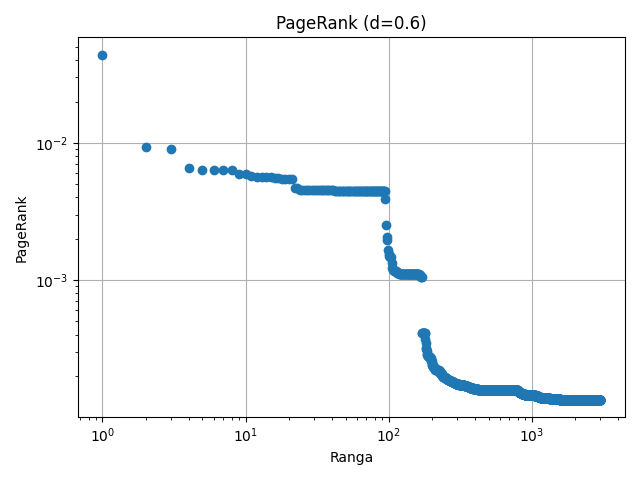
\includegraphics[width=0.6\textwidth]{assets/img_56.png}
\caption{Rozkład PageRank ($d=0.6$)}
\end{figure}

\textbf{Damping = 0.75}

\begin{itemize}
    \item Top 5 stron — max PR: 0.08237
    \item Regresja log-log: $x^{-0.71}$, $R^2 = 0.707$
\end{itemize}

\begin{figure}[H]
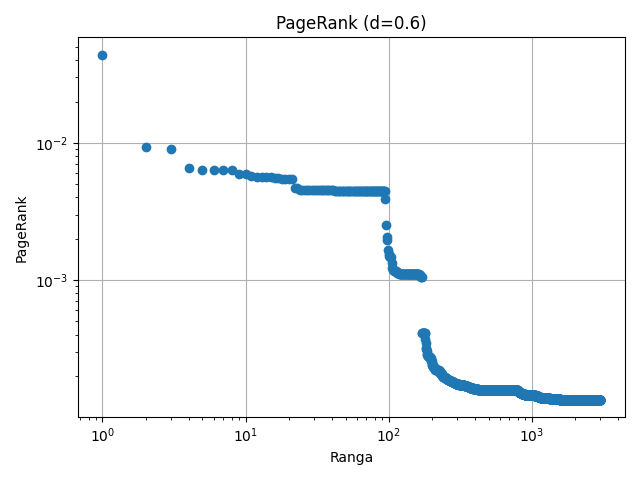
\includegraphics[width=0.6\textwidth]{assets/img_57.png}
\caption{Rozkład PageRank ($d=0.75$)}
\end{figure}

\textbf{Damping = 0.85}

\begin{itemize}
    \item Top 5 stron — max PR: 0.14197
    \item Regresja log-log: $x^{-0.83}$, $R^2 = 0.746$
\end{itemize}

\begin{figure}[H]
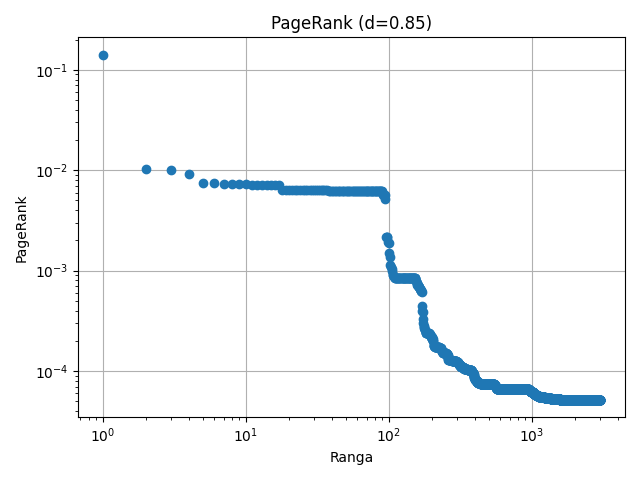
\includegraphics[width=0.6\textwidth]{assets/img_58.png}
\caption{Rozkład PageRank ($d=0.85$)}
\end{figure}

\textbf{Damping = 0.95}

\begin{itemize}
    \item Top 5 stron — max PR: 0.34959
    \item Regresja log-log: $x^{-1.04}$, $R^2 = 0.799$
\end{itemize}

\begin{figure}[H]
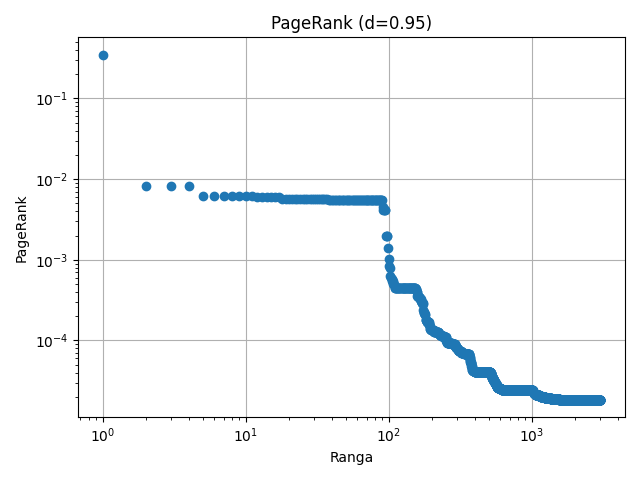
\includegraphics[width=0.6\textwidth]{assets/img_59.png}
\caption{Rozkład PageRank ($d=0.95$)}
\end{figure}

\textbf{Damping = 1.0}

\begin{itemize}
    \item Top 5 stron — max PR: 0.93913
    \item Regresja log-log: $x^{-1.67}$, $R^2 = 0.868$
\end{itemize}

\begin{figure}[H]
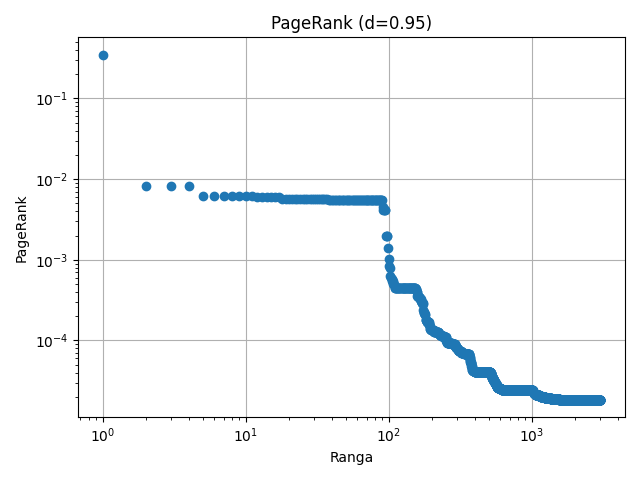
\includegraphics[width=0.6\textwidth]{assets/img_60.png}
\caption{Rozkład PageRank ($d=1.0$)}
\end{figure}

\subsection{Wnioski}

\begin{itemize}
    \item Wartości PageRank podlegają rozkładowi potęgowemu z dość wysokim współczynnikiem determinacji $R^2$ — potwierdza to typową dla sieci WWW właściwość skali bezwzględnej.
    \item Zwiększanie współczynnika tłumienia powoduje bardziej wyraźną hierarchizację — wyższe PR dla głównych stron, większe różnice pomiędzy liderami i resztą grafu.
    \item Najwyższe wartości PR osiągają strony główne domeny uczelni, strony polityki prywatności oraz podstrony pomocy i zasobów — co potwierdza skuteczność algorytmu PageRank w identyfikowaniu najważniejszych zasobów.
    \item Zbieżność rozkładu PR jest stabilna dla szerokiego zakresu wartości $d$, co świadczy o poprawności implementacji.
\end{itemize}
